\chapter{运行实例}

\begin{figure}[htbp]
\centerline{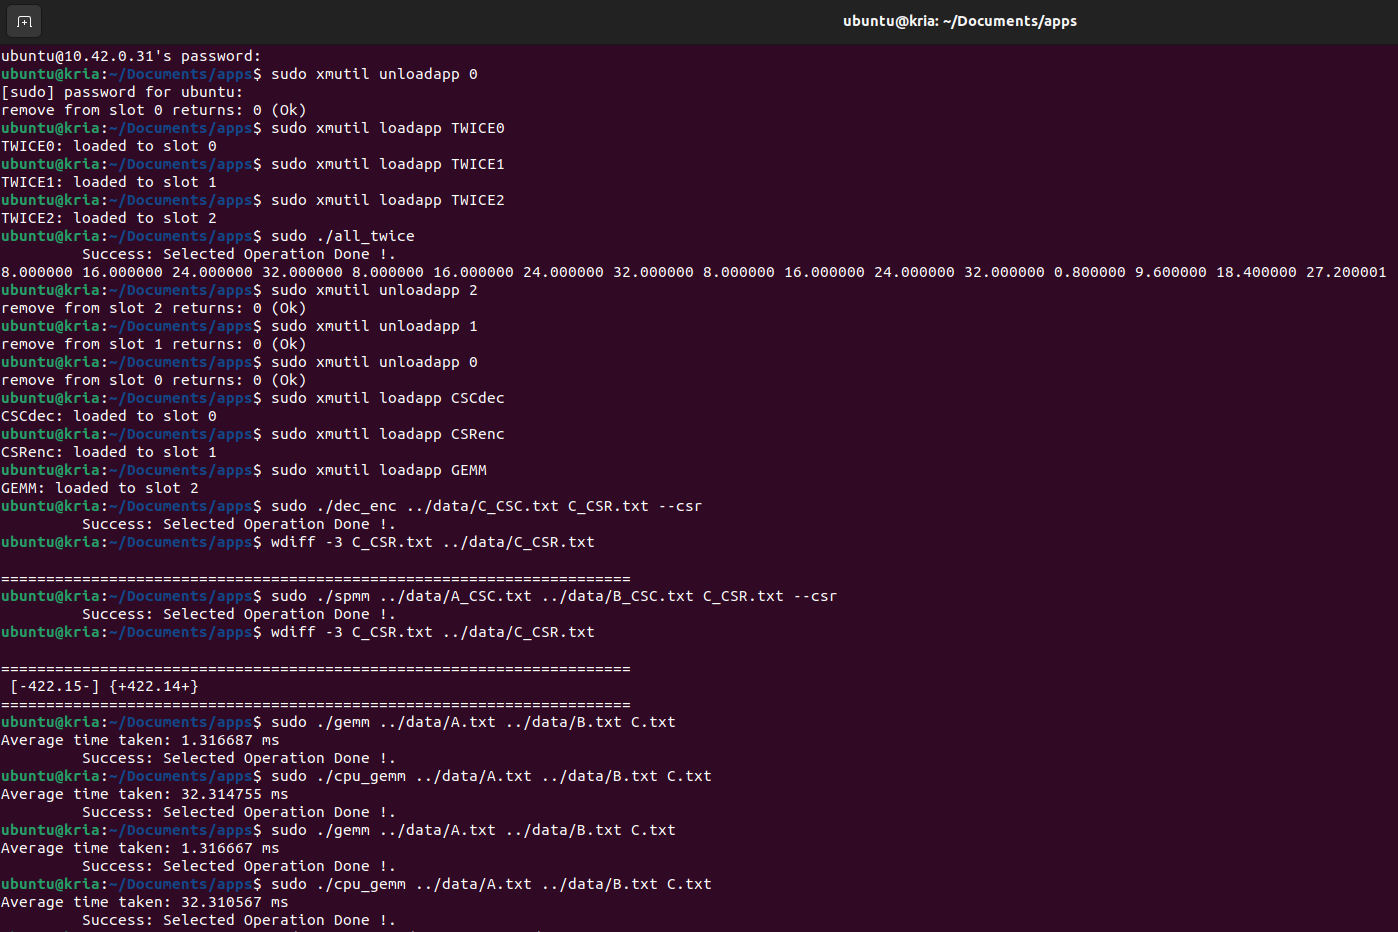
\includegraphics[width=\columnwidth]{figures/run.png}}
\caption{128\texttimes{}128矩阵乘法的运行实例。}
\label{fig:run}
\end{figure}

在图~\ref{fig:run} 中,我们先用 \verb|xmutil| 命令装载了三个 \verb|TWICE| RM,它们的功能是将输入流翻倍后输出。
我们随后执行 \verb|all_twice| 应用以测试RM间的互联,此应用定义RP\_0的输入为DDR,RP\_0输出为RP\_1的输入,
RP\_1输出为RP\_2的输入,RP\_2的输出为DDR,也就是将最开始的输入翻8倍后输出。

我们接下来卸载三个 \verb|TWICE| RM,装载 \verb|CSCdec|(CSC矩阵解压RM),\verb|CSRenc|(CSR矩阵压缩RM),\verb|GEMM|(稠密矩阵乘法RM)。
\verb|dec_enc| 应用将 \verb|CSCdec| 的输出连接 \verb|CSRenc| 的输入,实现CSC格式转化为CSR格式。\verb|spmm| 应用执行稀疏矩阵乘法,其输入为2个CSC矩阵,输出为CSR矩阵。
\verb|wdiff| 工具用于比对FPGA输出与真实值。\verb|gemm| 和 \verb|cpu_gemm| 应用分别测试FPGA和CPU上稠密矩阵乘法的运行耗时。

\chapter{稠密矩阵乘法加速}

\begin{table}[htbp]
\caption{不同矩阵大小下的加速比(12\texttimes{}12脉动阵列分块)}
\centering
\begin{tabular}{|c|c|c|c|}
\hline
\textbf{矩阵大小} & \textbf{CPU耗时} & \textbf{FPGA耗时} & \textbf{加速比} \\ \hline
12\texttimes{}12 & 0.015 & 0.012 & 1.3\texttimes{} \\ \hline
16\texttimes{}16 & 0.034 & 0.019 & 1.8\texttimes{} \\ \hline
32\texttimes{}32 & 0.26 & 0.047 & 5.5\texttimes{} \\ \hline
36\texttimes{}36 & 0.37 & 0.052 & 7.1\texttimes{} \\ \hline
60\texttimes{}60 & 1.7 & 0.17 & 10\texttimes{} \\ \hline
64\texttimes{}64 & 2.0 & 0.24 & 8.3\texttimes{} \\ \hline
96\texttimes{}96 & 7.3 & 0.56 & 13\texttimes{} \\ \hline
120\texttimes{}120 & 15 & 1.0 & 15\texttimes{} \\ \hline
127\texttimes{}127 & 17 & 1.3 & 13\texttimes{} \\ \hline
128\texttimes{}128 & 32 & 1.3 & 25\texttimes{} \\ \hline
\end{tabular}
\label{tab:speedup}
\end{table}

表~\ref{tab:speedup} 展示了对各种矩阵大小获得的加速比。CPU耗时从120\texttimes{}120至128\texttimes{}128矩阵乘法翻了一倍。
缓存未命中(Cache Miss)是影响其性能的关键因素,主要分为容量性未命中与冲突性未命中。
当矩阵维度\(N\)为2的幂次方(如128)时,对于行主序存储的矩阵\(B\),
在按列访问(计算\(B_{kj}\)时\(k\)递增)过程中,内存访问步长为 \(N\times\mathrm{sizeof(element)}\)。
若元素为4字节浮点数,\(N=128\)时的步长为512字节。
此类2的幂次方的步长极易与缓存的组索引机制(通常基于地址的低位比特)产生不良耦合,
导致同一数据流(如B矩阵的一列)中的多个缓存行映射到数量极为有限的缓存组上。
当这些并发访问的缓存行数量超过目标组的相联度时,将引发剧烈的缓存颠簸(Thrashing)。

与\(N=128\)的情形不同,当矩阵维度\(N=127\)时,其列访问步长并非2的幂次方。
这种非2的幂次方的步长使得内存地址在映射到缓存组时呈现出更优的分布特性,从而有效规避了因地址对齐引发的系统性缓存组冲突。
因此,尽管\(N=127\)的矩阵同样面临容量性未命中的挑战,但其性能表现显著优于\(N=128\)的情况,后者额外承受了严重的冲突性未命中负担。

\chapter{复现说明}

\begin{table}[htbp]
\caption{编译环境}
\centering
\begin{tabular}{lc}
\toprule
OS & Ubuntu 22.04.5 LTS \\
CPU & Intel Core i9-13900HX \\
Memory & 62.6 GiB \\
\bottomrule
\end{tabular}
\label{tab:env}
\end{table}

HLS代码由Vitis 2022.1综合成RTL IP,随后用Vivado 2022.1执行综合、实现和比特流生成,运行环境如表~\ref{tab:env} 所示。
在此环境下,Vivado流程需运行30分钟并占用55 GiB内存。若希望减小内存占用,可修改流程的并行线程数量。
同时,我们在 \url{github.com/fjtcin/dfx-3rp-bin} 提供了生成的二进制文件,可直接使用。
